\begin{center}
    PRACTICA DE LABORATORIO N° 02
\end{center}

\section{OBJETIVOS}
Crear relaciones automáticas y manuales

\section{REQUERIMIENTOS}

\begin{itemize}

- Conocimientos básicos de administración de base de datos Microsoft   SQL Server.
\\- Conocimientos básicos de SQL.
\\- Microsoft SQL Server 2016 o superior
\\- Base de datos AdventureWorks2016 o superior
\\- Power BI Desktop.
\\- Tener una cuenta Microsoft registrada en el Portal de Power Bi.
\end{itemize}

\section{DESARROLLO} 

\begin{itemize}
1. Ingresar a Power BI Desktop, en el cuadro de dialogo Obtener Datos (Get Data), asegurarse que Excel esta seleccionado y hacer click en Conectar (Connect), buscar el archivo Adventure Works Sales Data.xlsx y hacer click en Cargar (Load).

\end{itemize} 

\begin{center}
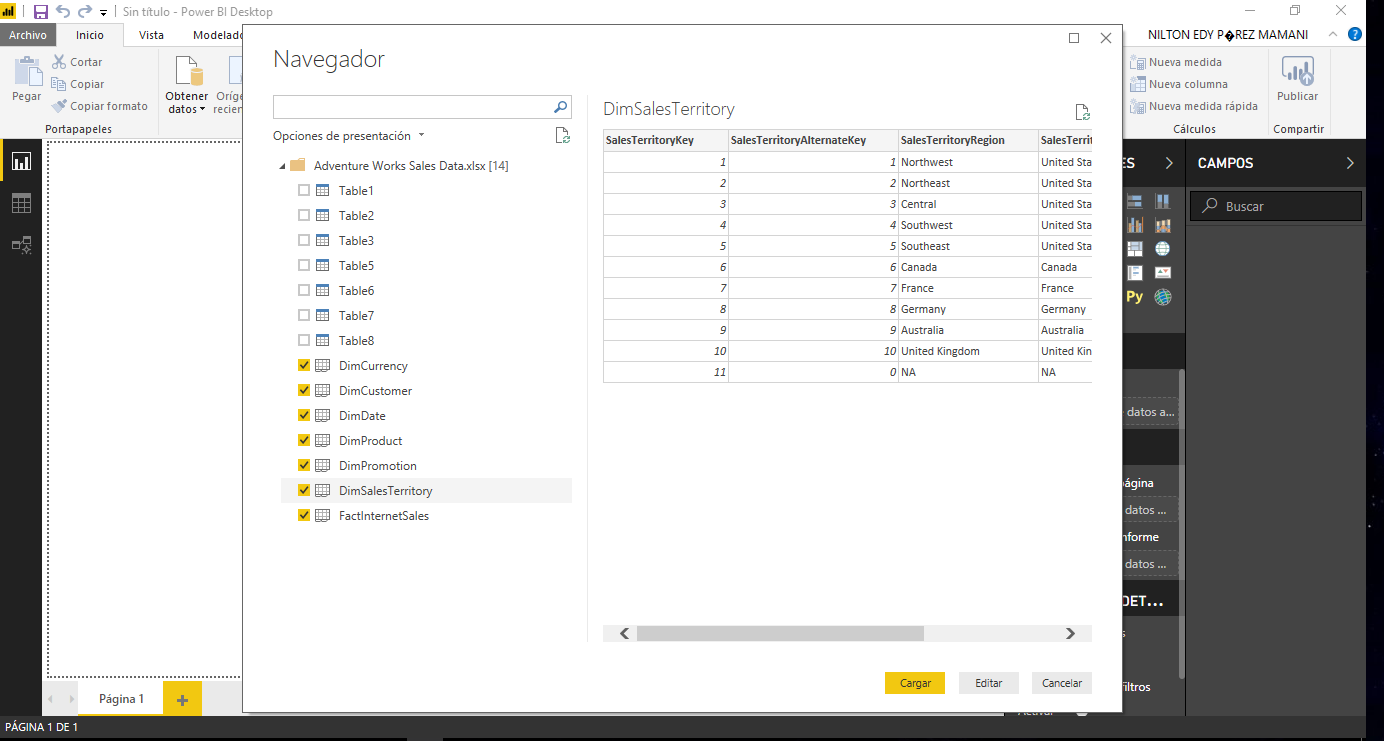
\includegraphics[width=15cm]{./Imagenes/img1} 
\end{center}

\begin{itemize}
2. En el cuadro de Administrar relaciones (Manage Relationships) realizar las configuraciones indicadas 
\end{itemize} 

\begin{center}
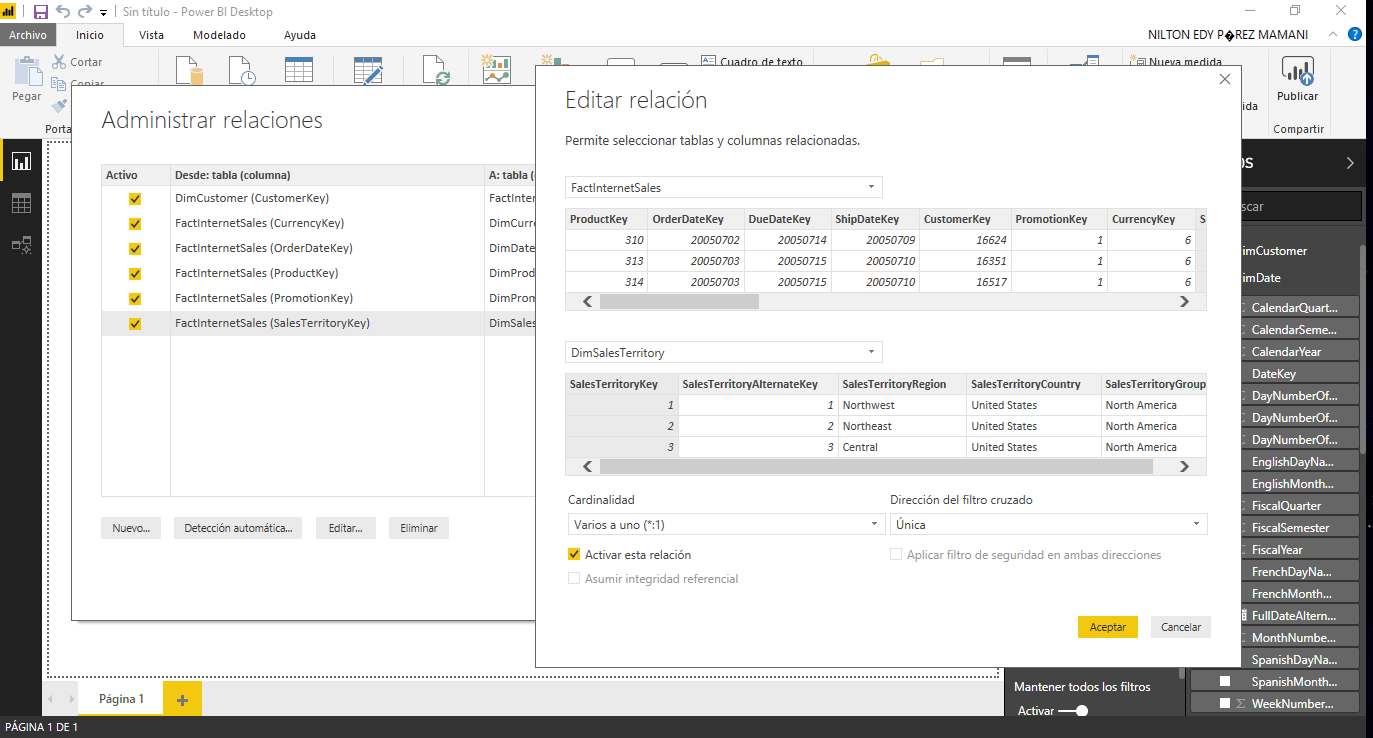
\includegraphics[width=15cm]{./Imagenes/img2} 
\end{center}

\begin{itemize}
3. En el cuadro de Administrar relaciones (Manage Relationships), hacer click en Nueva (New)y en la lista de tablas superior, hacer click en FactInternetSales. Luego hacer click en la columna
CustomerKey en la vista de datos previa, en la lista de tablas superior, hacer click en DimCustomer, y hacer click CustomerKey en la vista de datos previa.En la lista de Cardinalidad (Cardinality), hacer click en Muchos a Uno (Many to One (*:1)), y luego hacer
click en Aceptar (OK).

\end{itemize} 

\begin{center}
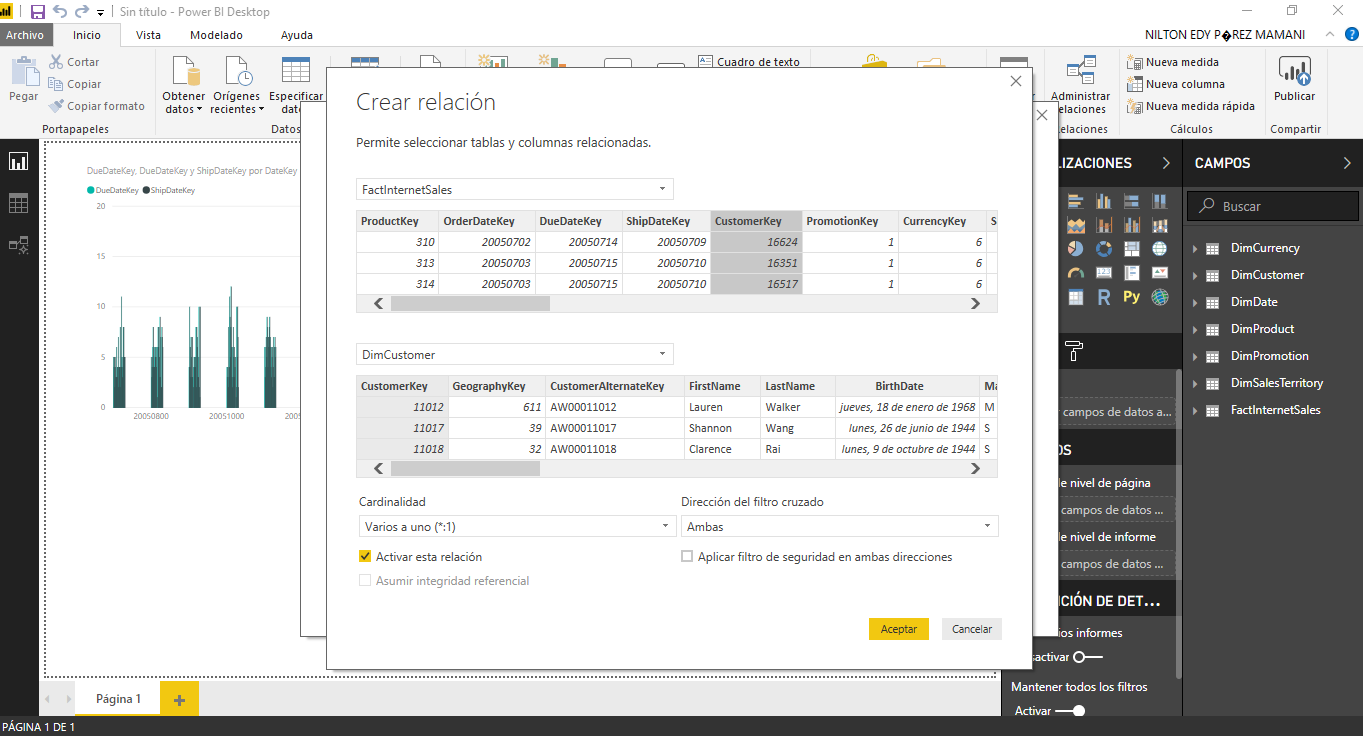
\includegraphics[width=15cm]{./Imagenes/img3} 
\end{center}

\begin{itemize}
4. Abrir el archivo Adventure Works Product Categories.xlsx
\end{itemize} 

\begin{center}
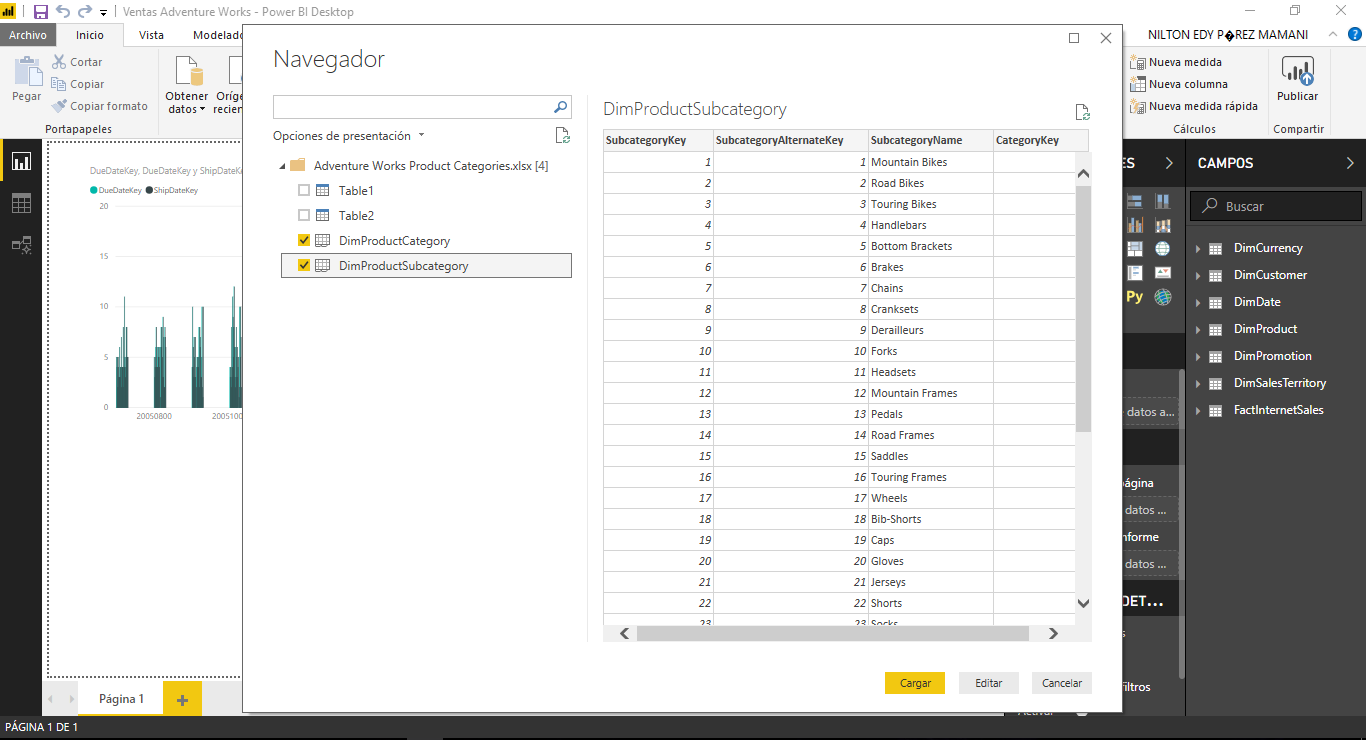
\includegraphics[width=15cm]{./Imagenes/img4} 
\end{center}

\begin{itemize}
5. En Power BI Desktop, haga clic en Datos en el panel de vistas en el lado izquierdo y realizar calculos agregando una nueva columna

\end{itemize}

\begin{center}
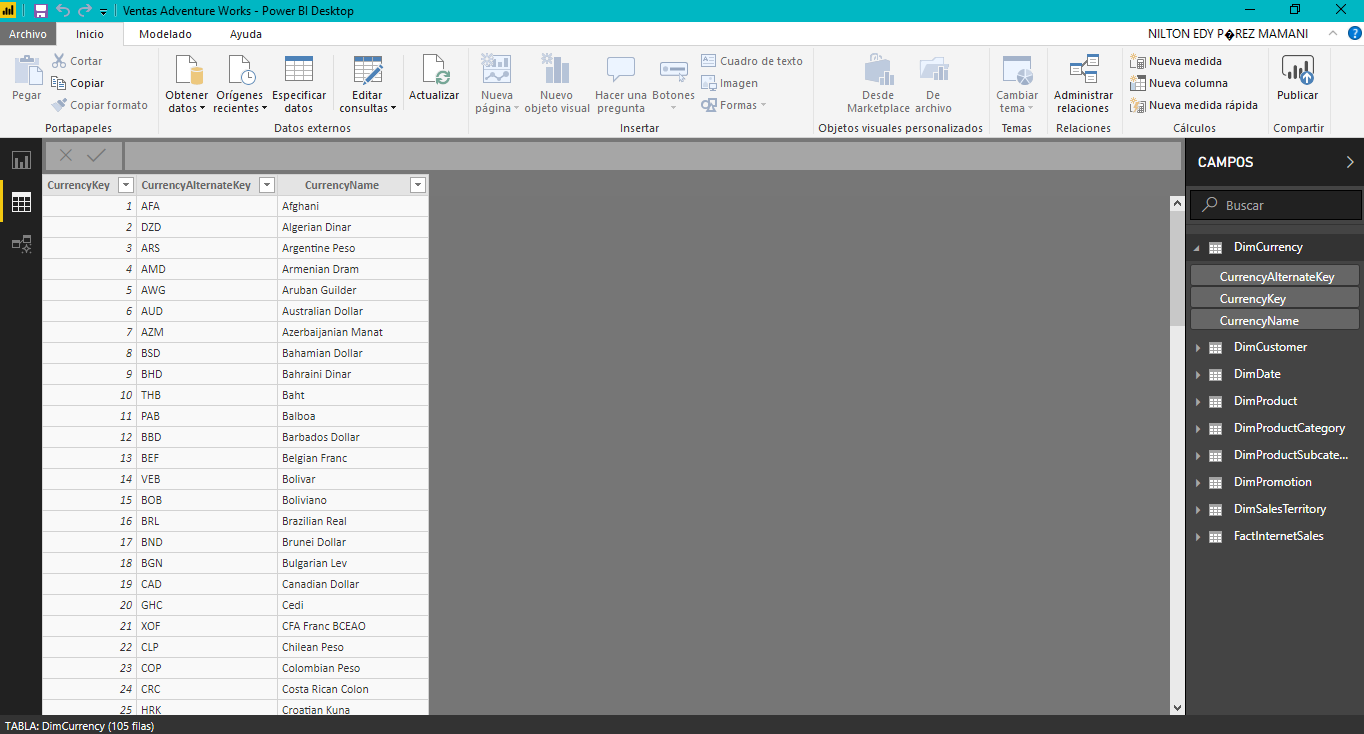
\includegraphics[width=15cm]{./Imagenes/img5} 
\end{center}

\begin{itemize}
6. En el panel Campos, haga clic en DimCustomer,en la cinta Modelado, en el grupo Cálculos, haga clic en Nueva columna.En la barra de fórmulas, resalte Columna = y escriba:
IncomeStatus = IF (DimCustomer[YearlyIncome] < 25000, "Lower Income",
IF (AND(DimCustomer[YearlyIncome] >= 25000, DimCustomer[YearlyIncome] < 60000),
"Middle Income",
IF (AND(DimCustomer[YearlyIncome] >= 60000, DimCustomer[YearlyIncome] < 100000),
"Higher Income",
IF (DimCustomer[YearlyIncome] >= 100000, "Very High Income", "Other")))) y finalmente presione Enter.
\end{itemize}

\begin{center}
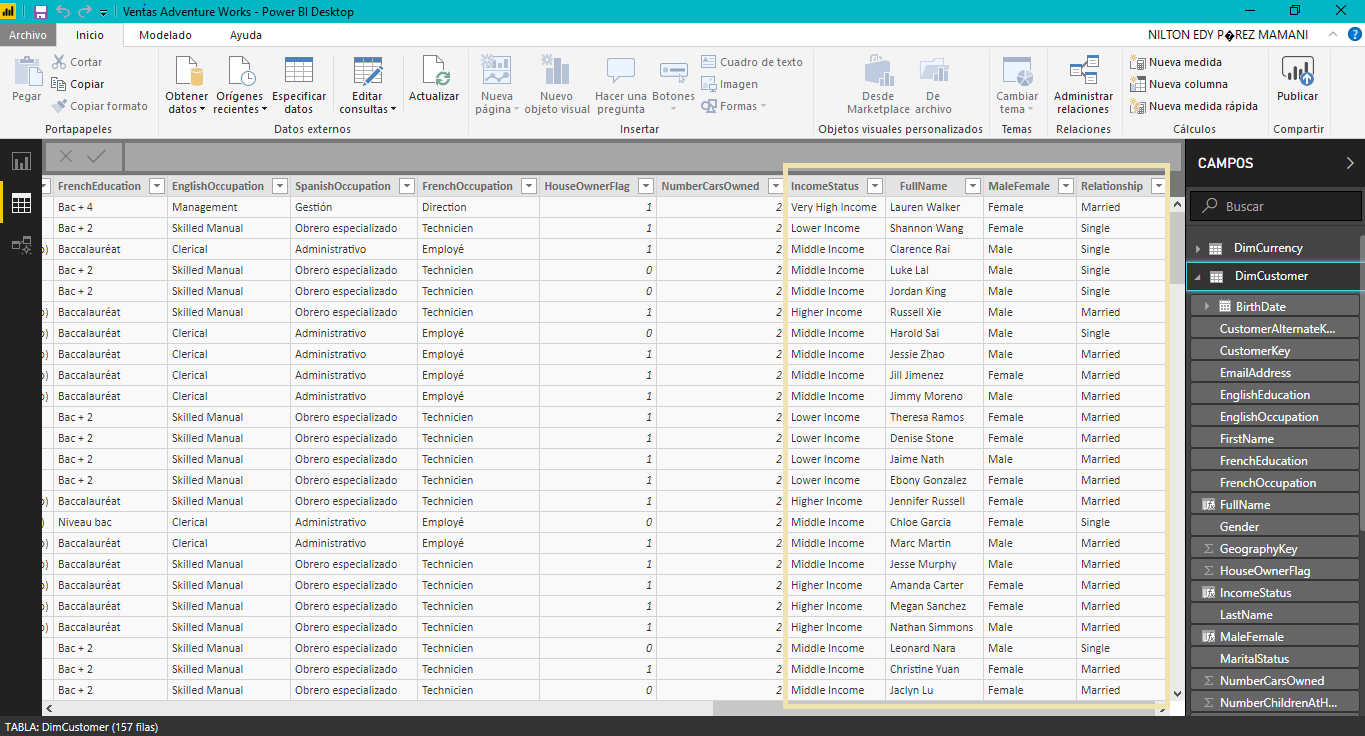
\includegraphics[width=15cm]{./Imagenes/img6} 
\end{center}

\begin{itemize}
7. En el panel Campos, haga clic en DimPromotion.En la cinta Modelado, en el grupo Cálculos, haga clic en Nueva columna y realizar la siguiente operacion:
PromotionLengthDays = DATEDIFF(DimPromotion[StartDate], DimPromotion[EndDate], DAY)


\end{itemize}

\begin{center}
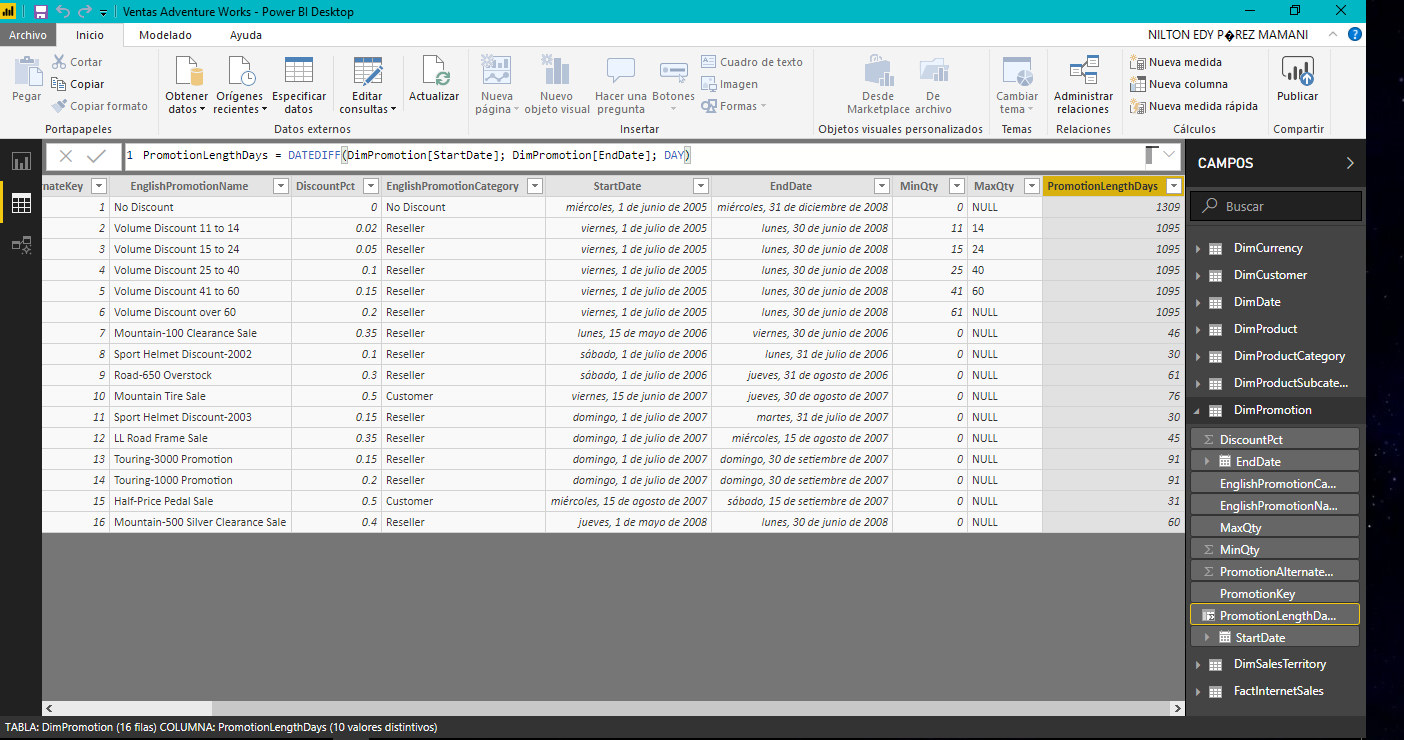
\includegraphics[width=15cm]{./Imagenes/img7} 
\end{center}


\begin{itemize}
8. En el panel Campos, haga clic en FactInternetSales.En la cinta Modelado, en el grupo Cálculos, haga clic en Nueva columna y realizar la siguiente operacion:
Profit = CURRENCY(FactInternetSales[UnitPrice] -
FactInternetSales[ProductStandardCost])
\end{itemize}

\begin{center}
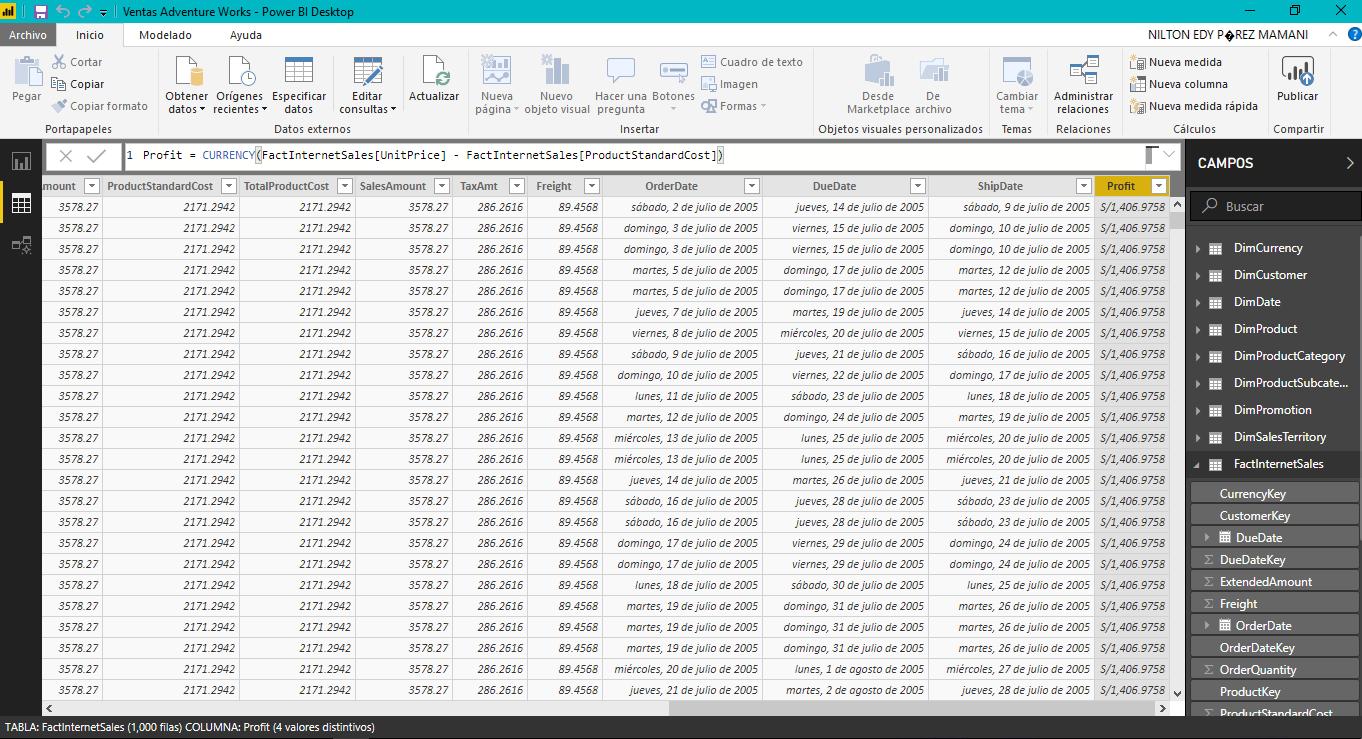
\includegraphics[width=15cm]{./Imagenes/img8} 
\end{center}